\section[Overall Description]{\hyperlink{toc}{Overall Description}}

\subsection[Product Perspective]{\hyperlink{toc}{Product Perspective}}
	Thanks to the general introduction and the scope definition of the system from the previous sections, we are now able to look at our system first from the outside and then from the inside. To deal with this description we are going to see the external interfaces of the system and then the definition of the model's structure in order to interact with them; at the end of the section \textbf{state diagrams} are used to emphasize the dynamic behavior of the most critical classes.
	\subsubsection[System Interfaces]{\hyperlink{toc}{System Interfaces}}
		\label{sec:systemInterfaces}
		SafeStreets offers an interface to its customers to provide them its basic and advanced functionalities. All the data needed to authenticate the users will be managed inside the system as well as the information related to the violations in order to be mined and crossed whenever needed.\\
		
		To accomplish the \hyperref[sec:goals]{\textcolor{blue}{goals}} stated in the \hyperref[sec:introduction]{\textcolor{blue}{introduction}} the application needs also to interact with three main external interfaces as reported in the following picture (\autoref{fig:systemInterfaces}).  
		\vspace{0,3cm}
		
		\begin{figure}[h]
			\centering
			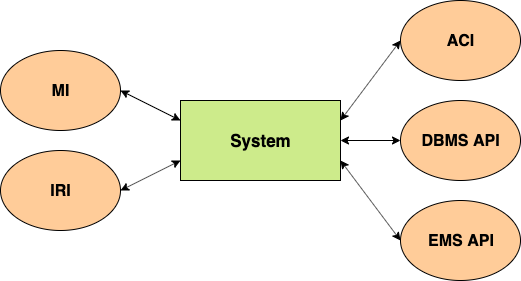
\includegraphics[scale=0.5]{externalInterfaces.png}
			\caption{\label{fig:systemInterfaces}System Interfaces}
		\end{figure}
		
		Two different kinds of interfaces are distinguished in the picture above:
		\begin{itemize}
			\item \textbf{Left hand side:} interfaces that provide functions (by means of APIs) for the system to perform internal operations. 
			
			In particular:
			\begin{itemize}
				\item \textsc{IRI} is used to process the image received from a violation. Whenever a violation is reported the system tries to recognize two distinct things from the picture helped by the additional data provided:
				\begin{itemize}
					\item \textbf{Plate:} the recognition of the plate's number is important to identify the vehicle by checking if it coincides with the one inserted or to add this information when missing. In both the cases when the number can not be identified the violation will be processed without it.
					\item \textbf{Type of vehicle:} is also very important to be recognized as the statistics can also be integrated with this filter. The vehicle will be reported without any type in case the process fails to find one, but we can assume that a shape recognition will be easily carried out by today's functionalities.
				\end{itemize} 
				\item \textsc{MI} is used to handle the geographical issues. The system needs to:
				\begin{itemize}
					\item \textbf{Retrieve} the name of the street where the violation occurred by using the provided position
					\item \textbf{Highlight} the safety of the streets and of municipality's areas
				\end{itemize}
			\end{itemize}
			\item \textbf{Right hand side:} interfaces that enable the system to send and receive data to the authorities. 
			
			In particular when:
			\begin{itemize}
				\item The reported violation has been accepted by the system and enriched with the metadata that can be useful for the authority. In this case the correct information is sent to the authority interested in the area that contains the related position.
				\item The municipality provides information about the accidents that occur in its area. Received data is crossed by the system to determine the safety of its streets. Thanks to this additional operation the application is also able to determine the best interventions for unsafe areas and suggest them to its users.
			\end{itemize}
		\end{itemize}
	
	\subsubsection[Model Structure]{\hyperlink{toc}{Model Structure}}
	The static analysis now continues to define the internal structure of the system, in particular with a high-level class diagram that shows the most important objects and their relations in order to achieve the \hyperref[sec:goals]{\textcolor{blue}{goals}}.\\
	
	The main objects in the UML diagram (\autoref{fig:classDiagram}) are:
	\begin{itemize}
		\item \textbf{Customer:} the system has to track two types of users. The distinction, in fact, is fundamental to recognize the municipality providing accident's data but also to give a different level of visibility to the information asked by a request.
		
		\item \textbf{User:} identifies a citizen with all the data he provides in its registration. Users are the clients of the application that report parking violations and look for \textbf{general} statistics related both to the frequency of parking violations in a street or to the safety of an area and its related suggested intervention.
		
		\item \textbf{Authority:} identifies the authority/municipality with all the data related to its recognition. Authorities are the clients of the application that receive the reported violations by the users but they also: ask for \textbf{specific} statistics and provide data about the accidents (crossed by the system).
		
		\item \textbf{Registration:} is used to authenticate the customer in order to perform actions he can only do recognized as a user or an authority.
		
		\item \textbf{Violation:} represents a general traffic violation. This class is thought to be used in a future extension of the system in case more violations are going to be considered.
		
		\item \textbf{ParkingViolation:} is the result of a notification provided by a user. In this way the application considers all the possible information that is filled whenever an infraction is reported. As we see in the UML diagram the class contains: multiple images for an  improved help to both the image recognition algorithm and the authorities; the position retrieved by the GPS (used to find the name of the street); the plate's number and all other metadata.
		
		\item \textbf{Accident:} will be used to store the data received by the municipality. No more specific description can be given here because only when interfacing with the municipality we will be able to know how the data has to be managed.
		
		\item \textbf{Position:} stores the coordinates of where the parking violation occurred. The position of each accident will be used to retrieve the street thanks to the functionalities provided by the MI and thus obtain statistics of each street and area.
		
		\item \textbf{Street:} is one of the most important object to be managed. Each recognized street will be added to the system to achieve its basic and advanced functionalities. A street considers also how many infractions happened in it; this is thought to simplify the very computing mining and crossing algorithms.
		
		\item \textbf{Area:} is another important object, in particular for the advanced functionality. An area contains the streets relative to its limits and is managed by the municipality that will receive all the violations reported in it. Areas are also critical for the safety they will encounter; to underline this we have defined an only method in the diagram (getSafety) that will be used later to define the related \textbf{state diagram}.
		
		\item \textbf{Vehicle:} vehicles are identified by the image recognition algorithm in order to provide additional information to the filter.
		 
		\item \textbf{Car:} are expected to be the most reported type of vehicles because of their dimensions and utilization (typically identified by the plate).
		
		\item \textbf{Motorcycle:} should be also considered as "critical" vehicles. The system has to care of particular areas where lots of motorcycles happen to be all parked in the wrong way and in uncomfortable spots.
		
		\item \textbf{Bicycle:} our system is supposed to deal also with bicycles. Obviously it will be much more difficult for the authorities to retrieve their owners but they can be used by the application to suggest possible interventions in the areas where they happen to be definitely cumbersome.
		
		\item \textbf{Request:} is the general class representing the interaction of a user with the system whenever statistics about the frequency, safety or suggestion is asked by the customer. In order to answer with the correct data it will be important to retrieve the user who sends the request to provide him the right visibility.
		
		\item \textbf{BasicRequest:} is the request that deals with the basic functionality. Thanks to it the application will be able to capture the filters selected by the user and answer correctly.
		
		\item \textbf{AdvancedRequest:} is the request that deals with the advanced functionality. Thanks to it the application will be able to capture the requirements of the customer, that in this case can be: the safety of a municipality's area or the suggestion for a possible intervention.
	\end{itemize}
	
	\begin{figure}[h!]
		\centering
		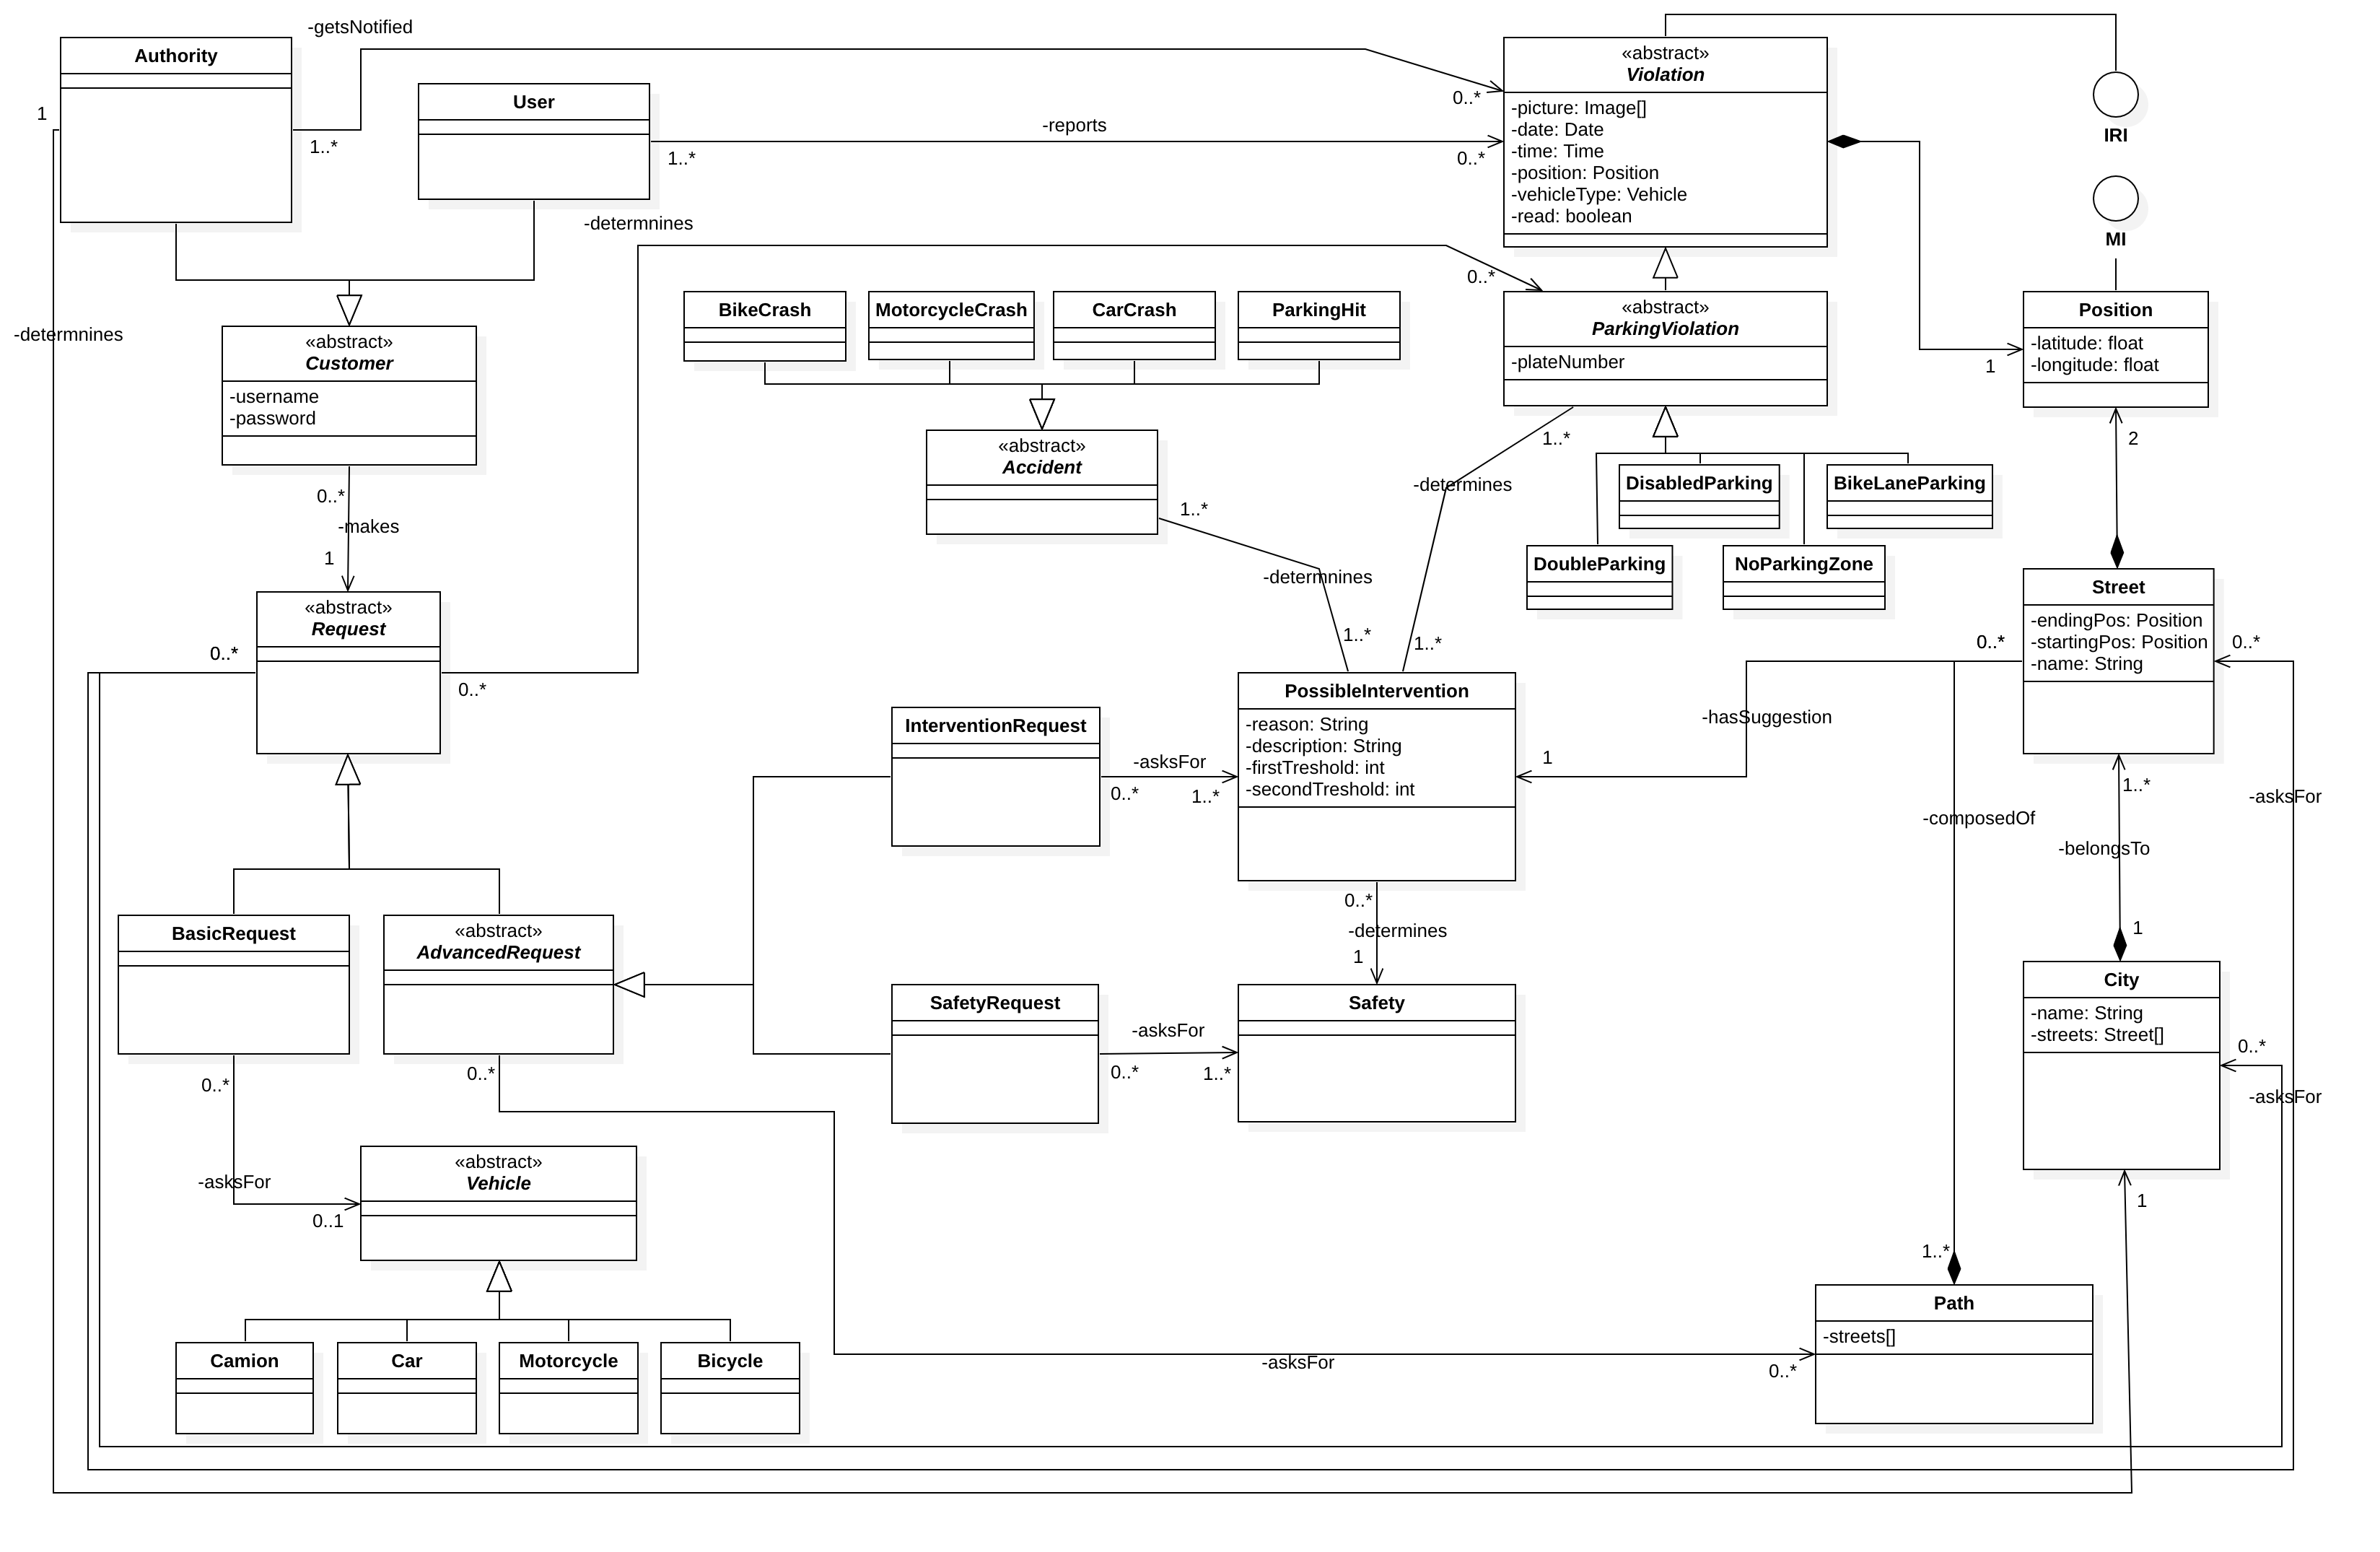
\includegraphics[width=\paperwidth - 1cm, angle=90]{/diagrams/classDiagramModel.png}
		\caption{\label{fig:classDiagram}High-level model structure}
	\end{figure}

	\FloatBarrier
	
	\subsubsection[State Diagrams]{\hyperlink{toc}{State Diagrams}}
	Considering now the main functionalities of the system, it is important to highlight the events that make its objects move from one state to another. State diagrams are used to describe the most critical aspects of the objects previously described in the UML class diagram (\autoref{fig:classDiagram}).
	
	\paragraph{Notification}
		Beginning with the notification of a parking violation it is important to remember that each infraction will be refused by the system i.i.f inconsistency is found; for example multiple images representing different types of vehicles.
		The diagram (\autoref{fig:notifyState}) starts when a violation is received in the \textit{unprocessed} state. First the system needs to check the consistency of the data received in order to accept or reject the violation. If the message is \textit{rejected} the notification diagram ends, otherwise the \textit{accepted} violation needs some more checks before it can be stored in the system. Second another check is used to understand if the infraction lacks of some important fields to be stored that however the application should be able to retrieve easily thanks to the functionalities provided by the external interfaces. Then, if the message is \textit{complete} it is ready to be enriched with other metadata (the name of the street retrieved by the GPS position), otherwise it is completed with missing information and then the \textit{ready} state is reached too. Lastly the information about the parking violation is \textit{stored}in the system, \textit{sent}to the authority and the notification diagram ends.
		
		\vspace{0.3cm}
		\begin{figure}[h]
			\centering
			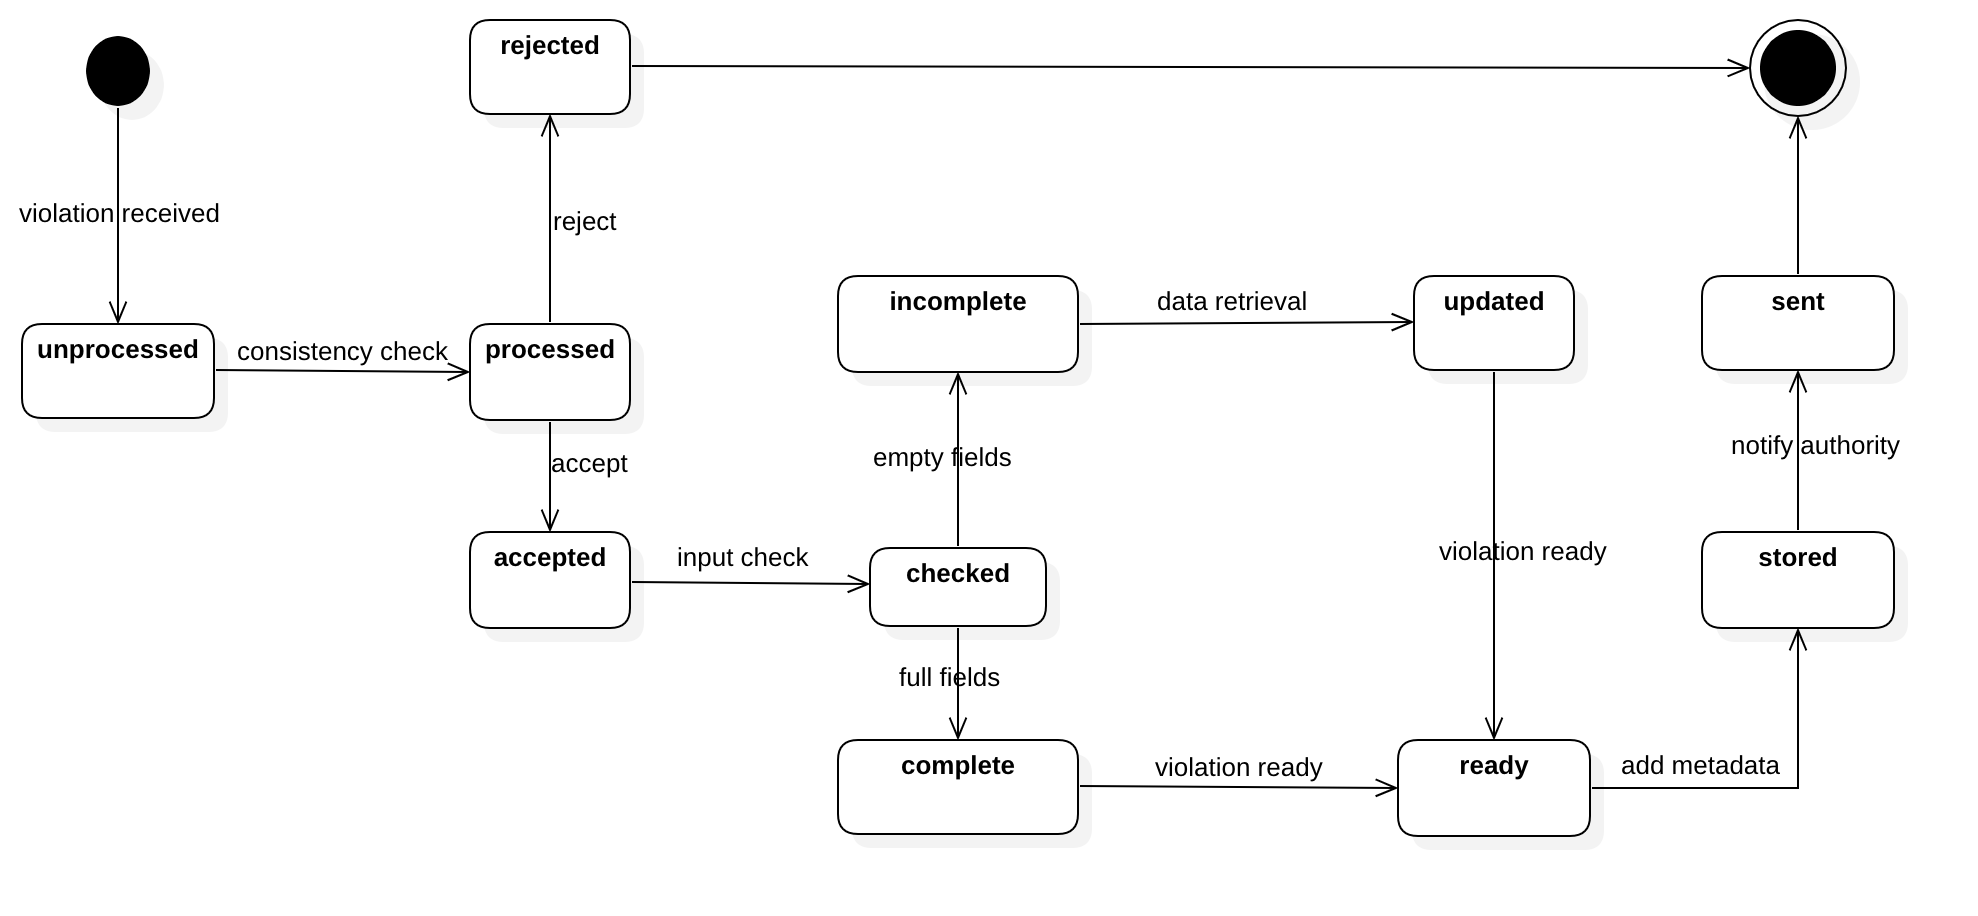
\includegraphics[scale=0.18]{/diagrams/state/notify.png}
			\caption{\label{fig:notifyState}Notification state diagram}
		\end{figure}
	
	\paragraph{Request}
		Statistics retrieval is another critical functionality that needs a state diagram in order to define how the information asked is provided with different levels of visibility depending on the role of the customer.
		The diagram (\autoref{fig:requestState}) represents both different kinds of requests a customer can do, in fact it is used to highlight the different visibility of the answered information rather than the difference between the requests. Whenever a query is received, the system has first to retrieve the data that is required thanks to the filters provided by the customer. After the information is found in the \textit{processed} state, the application needs to recognize the user in order to provide him the data with the level of visibility devoted to him. If the request comes from a user its data is filtered and once ready (\textit{user data} state), sent back to the user; symmetrically happens for the authority who will receive the least aggregate information possible. 
		
		\vspace{0.3cm}
		\begin{figure}[h]
			\centering
			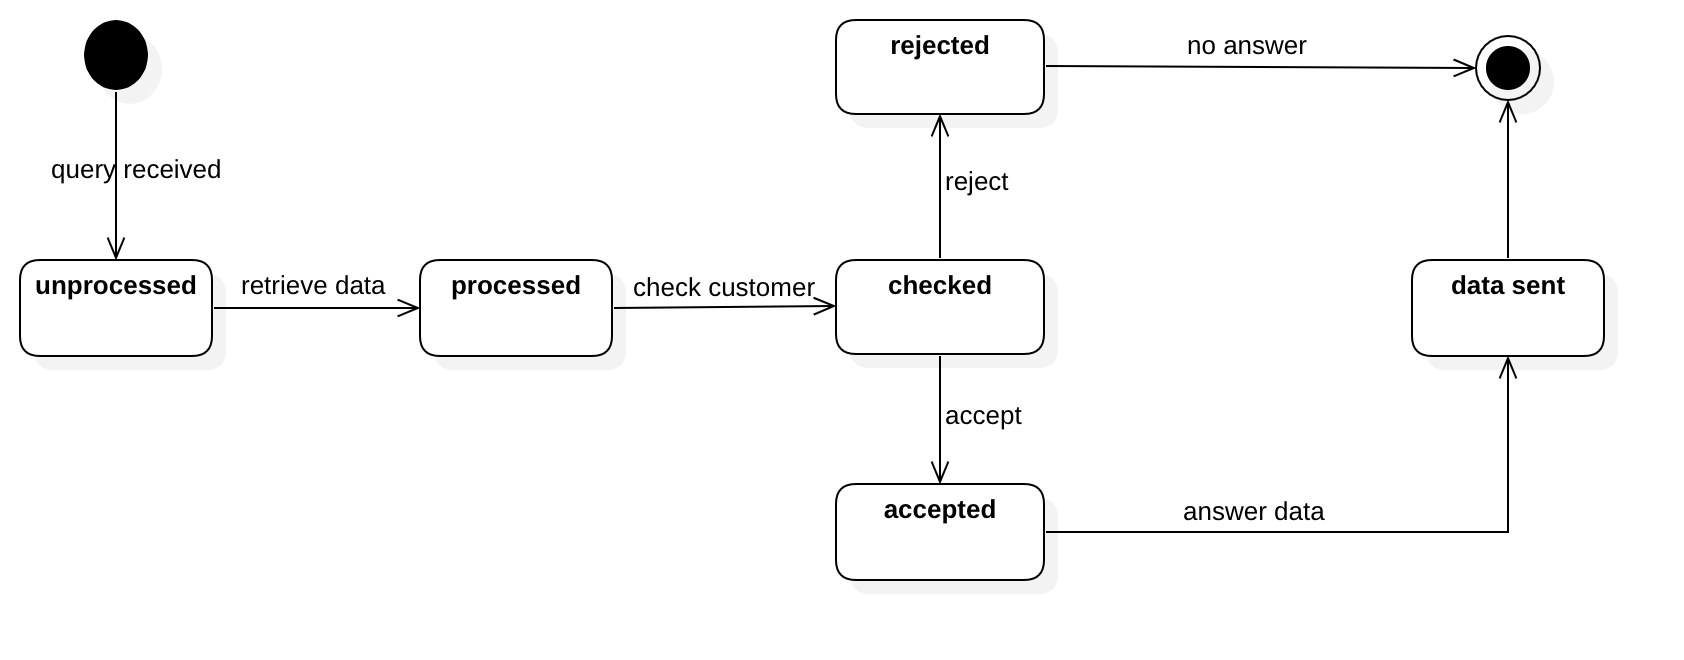
\includegraphics[scale=0.18]{/diagrams/state/request.png}
			\caption{\label{fig:requestState}Request for data state diagram}
		\end{figure}
	
	\paragraph{Safety}
		The last state diagram is used to highlight how the system is able to determine the safety of a street and update its state whenever new violations occur or new accidents data is provided by the municipality. 
		The diagram (\autoref{fig:safetyState}) shows how the safety of a street evolves in the time. The system is able to cross its own data with the one provided by the municipality to establish the safety of an area that will be evaluated thanks to some tresholds. At the beginning an area is considered \textit{safe} (and highlighted with the GREEN color) because no parking violation are stored and no cross can be performed. Once parking violations start to occur the application is able to keep track of their frequency and, thanks to the accidents information, will determine if the area has to be considered less safe than before or not. In this way once exceeded the safe treshold it will be considered \textit{half safe} (highlighted in YELLOW) and the same for the last state that represents an \textit{unsafe} area (highlighted in RED). Obviously the system has also to consider when an area enhances its safety; this will happen whenever one of the tresholds is not reached anymore. 
		
		\vspace{0.3cm}
		\begin{figure}[h]
			\centering
			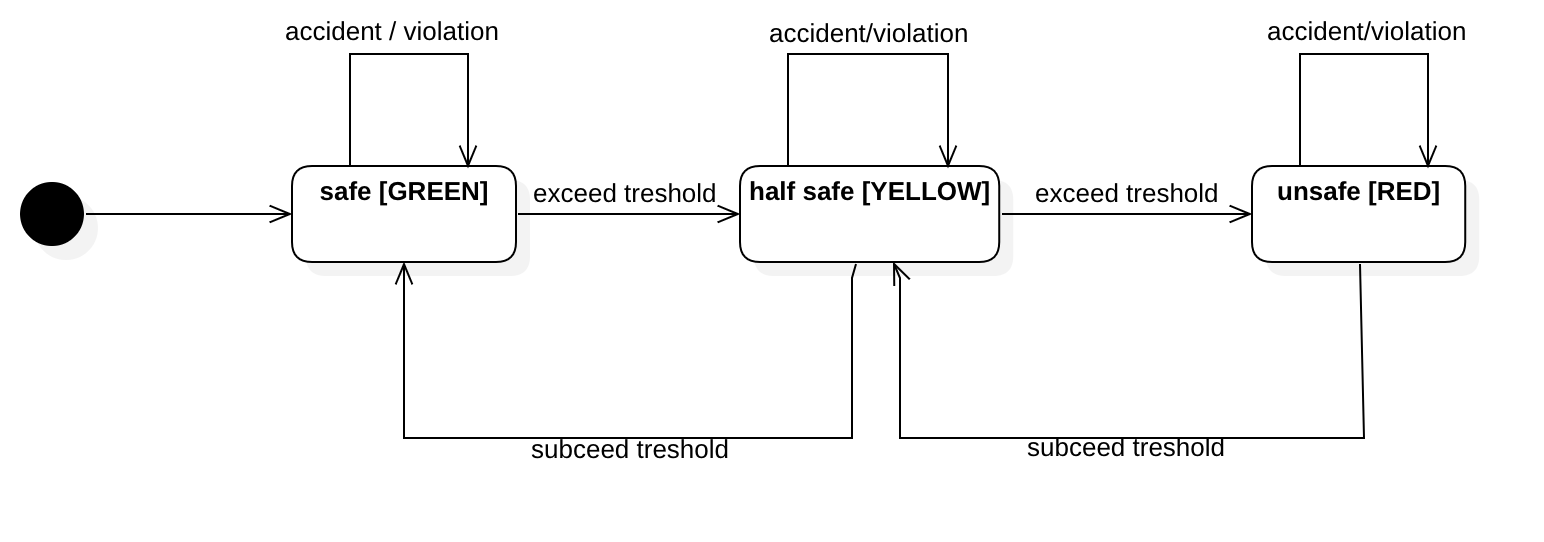
\includegraphics[scale=0.23]{/diagrams/state/safety.png}
			\caption{\label{fig:safetyState}Area safety state diagram}
		\end{figure}   

\subsection[Product Functions]{\hyperlink{toc}{Product Functions}}
	\label{sec:productFunctions}
	SafeStreet is a crowd-sourced application that intends to provide users with the possibility to notify authorities when parking violations occur. This has to be considered the main product function of the system because of its importance to obtain \textbf{crowdsourcing}. The information provided by users is what SafeStreet focuses on and what makes it able to provide services about the violations in a particular area. Thanks to mining and crossing processes, the system can find \textbf{statistics} and suggestions for interventions in unsafe areas. As the subsection is structured, the product functions will be precisely described following the same order of how we have just shallowly presented: first the \textbf{notification} function then the \textbf{statistics} one and in the end \textbf{safety}.
	
	\subsubsection[Notification Function]{\hyperlink{toc}{Notification Function}}
		\label{sec:notificationFunction}
		Users are allowed to notify authorities thanks to SafeStreets. First it is important to highlight that this functionality is allowed only to users that are logged-in to the system and thus recognized. Second, to improve the possibility of reporting a parking violation, the application provides a way to complete the notification not mandatory when the user takes the pictures of the infraction. In this way it is possible to report infractions even by users that are in a hurry or without enough battery to fill all the fields. This possibility allows also to consult the street law in order to decide if the violation is against the rules or to take every further consideration before reporting.\\
		
		The notification functionality is provided to the user by an interface that allows him to insert all the information needed to report a parking violation. The fields a user fills are reported here with a label that describes if they are mandatory or not.
		
		\begin{itemize}
			\item \textbf{Pictures}\texttt{[MANDATORY]:} users must provide at least one picture of the parking violation in order to report it. In this way it is possible to reduce the number of irregular notifications as the recognition functions will immediately discard pictures that do not contain any vehicle. Thanks to the possibility of inserting multiple images the application will be able to find easily the number of the plates and the type of the vehicles, obviously discarding all the notifications that contain inconsistent pictures.
			
			\item \textbf{Date}\texttt{[OPTIONAL]:} this field is considered optional because not fundamental for the functionalities of the system. Moreover it can be very useful crossed with the time to understand if the user has reported the violation as soon as the system receives it. In this case the violation it is promptly notified to the authority giving her the possibility take action immediately.
			
			\item \textbf{Time}\texttt{[OPTIONAL]:} like the date it can be used to understand if the user notifies the infraction as soon as he spots it. In addition this field is also used to provide a filter in the statistics functionality: a user can provide the timestamp when the violation occurred even later when he does not remember the precise time, in order to accomplish this functionality.
			
			\item \textbf{Position}\texttt{[MANDATORY]:} users must pin the place where the parking violation occurred in order to report it. SafeStreet's functionalities are based in fact on this information that is processed with the functionalities provided by the MI. As all the notifications the position can be pinned even later and will be used by the application to find the exact street where the parking infraction was spotted.
			
			\item \textbf{Type}\texttt{[OPTIONAL]:} users are optionally able to give additional information by providing the type of the violation they are reporting. This kind of data can be very useful for the authority that can decide in this way on which of all the notifications it receives to take action.
			
			\item \textbf{Plate}\texttt{[OPTIONAL]:} this field is thought to give additional information to the functionalities provided by the IRI in order to recognize the plate of the reported vehicle. Obviously it will be always discarded when the algorithm recognizes a vehicle that does not have a plate and in case inconsistency is found when matching it with the one recognized in the picture. Whenever a plate is not found, the violation will be stored and notified to the authority without this information. 
		\end{itemize}
	
		Once the violation is received, before storing it, the system: checks if all the mandatory fields are present, checks if no inconsistency is found in the provided information, adds the metadata relative to the type of violation and the street where the infraction occurred. After all the information relative to a parking violation is stored in the system the related notification is sent to the authority. %todo aggiungere la storia che ciascun polizziotto ha il suo dispositivo e così è in grado di agire subito, fare attenzione al fatto che bisogna controllare se la violazione è stata riportata prima o dopo. La product function relativa sarebbe dopo questa
		
	\subsubsection[Statistics Function]{\hyperlink{toc}{Statistics Function}}
		Data mining is used to retrieve the information about the stored data and provide the customers different ways to filter it. Thanks to the details of each infraction, in fact, the system is able to offer this service both to users and authorities. Customers, once decided the street of their interest, choose how to retrieve the frequency of parking violations by selecting the following filters:
			
		\begin{itemize}
			\item \textbf{No Filter:} the frequency is retrieved by giving a general view of all the parking violations that occur in the previously chosen street.
			
			\item \textbf{Time:} customers are able to filter the frequency by choosing a time lapse in which they are interested in. In this way the statistics can give very useful information both to users and authorities about the periods of time when the most violations occur.
			
			\item \textbf{Type of vehicles:} the system is able to understand the type of the reported vehicles thanks to the functionalities provided by the image recognition algorithms. In this way the information stored about each violation can be filtered choosing one of the recognized vehicles: \textbf{cars, motorcycles, bicycles}.
			
			\item \textbf{Type of violation:} thanks to the information about the type of the parking violation (typically provided by the user) the application allows also to filter by the type the frequency of the parking violations. We can think of this statistic mainly for the authorities who will look for the highest type of vehicles that commit a violation in a street in order to take action; however this filter is also allowed to users who may be interested in this kind of data too.
		\end{itemize}
	
	It is important to underline the fact that data is provided to each customer depending on its role. \textbf{Different levels of visibility} have to be considered when providing the information. For example: whenever an authority looks for the frequency in a street, it also receives a list of all the plates of the vehicles that committed those violations; users, instead, receive only the statistics in numbers. 
	
	\subsubsection[Safety Function]{\hyperlink{toc}{Safety Function}}
		SafeStreets is able to process the information about the accidents that occur on the territory of the municipality that provides this data. Thanks to this additional information the system can cross it with its stored one and determine the safety of each area. In order to choose if an area is safe or not, two tresholds have to be defined as three levels of safety can be highlighted: \textbf{safe}, \textbf{half-safe} and \textbf{unsafe}.\\
		
		The system dynamically changes the safety of an area thanks to the tresholds and uses this information to provide the customers two services related to the safety:
		
		\begin{itemize}
			\item \textbf{Colored Areas:} customers are able to retrieve the information about the safety of an area both in general or in a specified time slot. In order to distinguish the different types of safety previously described the application highlights the areas with:
			\begin{itemize}
				\item \textbf{GREEN:} safe area
				\item \textbf{YELLOW:} half-safe area
				\item \textbf{RED:} unsafe area
			\end{itemize} 
		
			\item \textbf{Intervention:} SafeStreets is also able to suggest a possible intervention only for the areas that are marked as unsafe. Customers are allowed to select an unsafe area and retrieve all the details for the intervention suggested; both users and authorities can access this functionality that is thought for: provide authorities the best solution in order to enhance the safety of the selected area; inform the users of the possible interventions that would be going to occur in the selected area if the municipality decides to take action.
		\end{itemize}
		
\subsection[User Characteristics]{\hyperlink{toc}{User Characteristics}}
	SafeStreets has two different customers that are very important to distinguish in order to provide correctly the functionalities previously described in subsection \ref{sec:productFunctions}. In the entire document a general client is called \textbf{customer} and the distinction is made between:
	
	\begin{itemize}
		\item \textbf{USER}
			\begin{itemize}
				\item Is considered to be reliable.
				\item Must have a smartphone to take pictures of a parking violation.
				\todo{Must be at least 16 years old ?}
				\item Can register to SafeStreets in order to be recognized as such.
				\item Must login to SafeStreets to notify a parking violation.
				\item Must login to SafeStreets to retrieve statistics.
				\item Can retrieve the safety of an area.
				\item Can retrieve the suggestion for an intervention of an unsafe area.
			\end{itemize}
		\item \textbf{AUTHORITY/MUNICIPALITY}
			\begin{itemize}
				\item Is considered to provide correct and reliable information about accidents.
				\item Can register to SafeStreets in order to be recognized as such.
				\item Must login to SafeStreets to retrieve statistics.
				\item Can provide information about the accidents that occur in its territory.
				\item Can retrieve the safety of an area.
				\item Can retrieve the suggestion for an intervention of an unsafe area.
			\end{itemize}
	\end{itemize}
	
\subsection[Domain Assumptions]{\hyperlink{toc}{Domain Assumptions}}
	\label{sec:domainAssumptions}
	Domain assumptions are used to define clearly the world in which SafeStreets interfaces. Thanks to them we are able to add constraints that define the bounds of the environment. \\
	
	We assume that these assumptions hold true in the domain of the system:
		
	\begin{enumerate}[label=\textbf{DA\arabic*}]
		\item GPS position is accurate ($\pm5$m).
		\item Users are reliable.
		\item Inconsistent and incomplete (with respect to the mandatory fields defined in \ref{sec:notificationFunction}) data received by the system is discarded.
		\item Information provided by the municipality is correct and reliable.
		\item The municipality area is composed of all the streets inside its limits.
	\end{enumerate} 
	
\subsection[The World and the Machine]{\hyperlink{toc}{The World and the Machine}}
	Thanks to the constraints on the domain of interest for the system (section \ref{sec:domainAssumptions}), we are now able to describe SafeStreets with the \textit{World and the Machine} approach that allows to underline the most important phenomena that are present in the problem we are dealing with. The machine represents the system do be developed while the world (a.k.a environment) is the portion of the real world affected by the machine.\\
	
	Thanks to the distinction we have highlighted in the next page (\autoref{fig:worldAndMachine}) the main phenomena of our problem: the ones in the world affect the world only, the ones in the machine affect the machine only and the ones in between affect both the world and the machine. This figure can be also used to start guessing the requirements (section \ref{sec:specificRequirements}) of our system as they can be defined as: \textit{prescriptive assertions formulated in terms of shared phenomena.} 
	
	\begin{figure}[h]
		\centering
		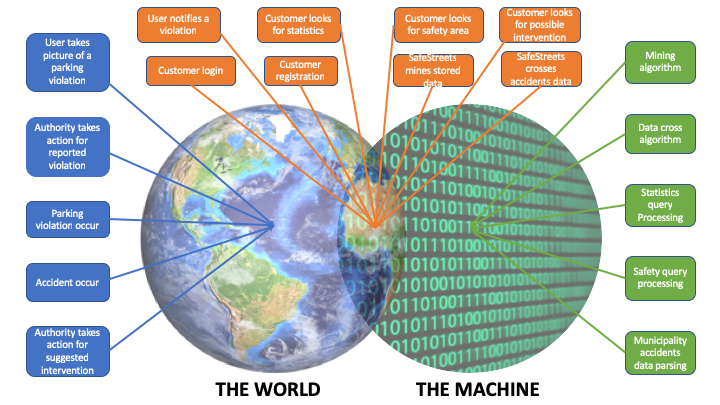
\includegraphics[angle=90, scale=0.6]{WorldAndMachine.png}
		\caption{\label{fig:worldAndMachine}The World and the Machine}
	\end{figure}
 